\section{The cosh ladder}\label{mi:sec:ladder}

The universal factor experiments of Section~\ref{mi:sec:miyatake} point to a constructive use of the same idea. For real $b$ let
\begin{equation}\label{mi:eq:Fb}
F_b(z)=\int_{-\infty}^\infty\Phi(u)\cosh(bu)e^{izu}\,du=\tfrac12\big\{\Xi(z+ib)+\Xi(z-ib)\big\},
\end{equation}
which is entire for every $b$ because $\Phi$ decays double exponentially, even, real on $\R$, of order one, and satisfies $F_b(0)=2\int_0^\infty\Phi\cosh(bu)\,du>0$. With $\alpha=\frac12+b$ and the variable $z$ real, $F_b(z)=\re\xi(\alpha+iz)$; in the notation of Section~\ref{pol:sec:cosh} it is $A_\alpha(iz)$.

\begin{theorem}[de Bruijn, Lagarias]\label{mi:thm:ladder}
For every $b\ge\frac12$ all zeros of $F_b$ are real, and $s\mapsto F_b(0)/F_b(i\sqrt s)$ is the Laplace transform of a generalised gamma convolution with Thorin measure $\sum_j\delta_{\gamma_j(b)^2}$, where $\pm\gamma_j(b)$ are the zeros of $F_b$. This holds unconditionally.
\end{theorem}

The statement is Theorem~\ref{pol:thm:cosh}(ii) and Corollary~\ref{pol:cor:evenpart} of Section~\ref{pol:sec:cosh} (the simplicity of the zeros is Lagarias's theorem \cite{Lagarias05}); we keep the proof, which is short.

\begin{proof}
The zeros of $\Xi$ lie in $|\im z|<\frac12$, the critical strip. By de Bruijn's strip theorem \cite{deBruijn}, all zeros of $\Xi(z+ib)+\Xi(z-ib)$ then lie in $|\im z|\le(\max(\frac14-b^2,0))^{1/2}$, so they are real for $b\ge\frac12$. Since $F_b$ is even of order one, Hadamard gives $F_b(z)=F_b(0)\prod_j(1-z^2/\gamma_j(b)^2)$ with $\sum_j\gamma_j(b)^{-2}<\infty$. Hence $F_b(0)/F_b(i\sqrt s)=\prod_j(1+s/\gamma_j(b)^2)^{-1}$, the Laplace transform of $\sum_je_j/\gamma_j(b)^2$ with independent standard exponentials $e_j$.
\end{proof}

Let $B_{\cosh}=\inf\{b\ge0:\ F_b\text{ has only real zeros}\}$. Then $B_{\cosh}\le\frac12$ unconditionally, and $B_{\cosh}=0$ if and only if $\RH$ holds: $\RH$ gives $B_{\cosh}=0$ because $F_0=\Xi$, and conversely if $F_{b_n}$ is real rooted along a sequence $b_n\downarrow0$, which exists because $B_{\cosh}$ is an infimum, Hurwitz's theorem passes real rootedness to the limit $\Xi$. The set of real rooted $b$ need not be an interval, and the argument does not use that. So $\RH$ is the statement that the ladder of Theorem~\ref{mi:thm:ladder} reaches the bottom rung. The constant $\Omega$ of Chapter~\ref{chap:ferro} is defined through ferromagnetic cosine tilts for every $a\ge a_0$; both constants are at most $\frac12$ and both vanish under $\RH$. Two remarks fix the place of the ladder in the Thorin programme.

The first concerns the space below the bottom. Dividing by $\cosh(bu)$ instead of multiplying, the transform $g_b$ of Section~\ref{mi:sec:prob} has nonreal zeros at a height that recedes as $b\to0$, in every case computed (Section~\ref{mi:sec:miyatake}); for Gaussian factors the corresponding statement is the theorem of Rodgers and Tao \cite{RodgersTao}. If $\RH$ holds, $\Lambda=0$ by their theorem, so along the de Bruijn Newman flow the reciprocal $\Xi$ sits at the edge of the generalised gamma convolution class.

The second concerns computation. One might hope to lower the unconditional bound $B_{\cosh}\le\frac12$ in the spirit of the Polymath bound \cite{Polymath} for the de Bruijn Newman constant. Section~\ref{mi:sec:quasi} proves $B_{\cosh}\le\sigma_{\max}-\frac12$, with $\sigma_{\max}$ the supremum of the real parts of the zeros, and that the paired version of the ladder bottoms out exactly at $\sigma_{\max}-\frac12$; it conjectures that lowering $B_{\cosh}$ is, at large height, a quasi Riemann hypothesis (Conjecture~\ref{mi:conj:quasi}). Any zero free half plane $\re s>\sigma_0$ gives $B_{\cosh}\le\sigma_0-\frac12$; the half plane $\re s>\frac78$ announced in October 2026 and recorded in Chapter~\ref{chap:ferro} would give $B_{\cosh}\le\frac38$.

\section{Miyatake's identity, read probabilistically}\label{mi:sec:prob}

Throughout this and the next two sections $\Phi$ is the kernel of Section~\ref{mi:sec:miyatake}, with $\Xi(z)=\int_\R\Phi(u)e^{izu}\,du$; it is even, positive, analytic in $|\im u|<\pi/4$ and decays like $\exp(-\pi e^{2|u|})$. For $b>0$ put
\[
g_b(z)=\int_\R\Phi(u)\sech(bu)\,e^{izu}\,du ,
\]
the transform of $\Phi/\cosh(bu)$ studied in Section~\ref{mi:sec:miyatake}. It is entire of order at most one, even and real on $\R$, and Miyatake's transform of $\psi_{\mathrm M}$ is $g(x)=G_{\mathrm M}(ix)=g_{9/2}(2x)/(4\pi^2)$.

\begin{proposition}[Shift identity]\label{mi:prop:shiftb}
For every $b>0$ and $z\in\C$, $\Xi(z)=\frac12\{g_b(z+ib)+g_b(z-ib)\}$, that is $\Xi=\cos(b\partial)g_b$ with $\partial=d/dz$. Miyatake's identity \eqref{mi:eq:miyid} is the case $b=\frac92$.
\end{proposition}

\begin{proof}
Write $\Phi=\Phi\sech(bu)\cdot\frac12(e^{bu}+e^{-bu})$; the integrals converge for all $z$.
\end{proof}

So $g_b=\sec(b\partial)\Xi$ is $\Xi$ pushed backwards through the universal factor $\cos(b\partial)$, which is why $Q$ decreases while universal factors increase. Three classical objects describe the inverse map. Let $\mathcal H_\lambda(z)=\int_\R\Phi(u)e^{\lambda u^2}e^{izu}\,du$ be the de Bruijn Newman family in the normalisation of this chapter; in that of Section~\ref{sec:ch21:flow}, $H_t(z)=\frac18\mathcal H_{t/4}(z/2)$.

\begin{theorem}[L\'evy area, P\'olya Gamma clock, Thorin atoms]\label{mi:thm:levyarea}
Let $\mathcal A=\frac12\int_0^1(W^1dW^2-W^2dW^1)$ be L\'evy's stochastic area of a planar Brownian motion $(W^1,W^2)$, with $\E e^{i\lambda\mathcal A}=\sech(\lambda/2)$, and let $\varpi\sim\mathrm{PG}(1,0)$ be a P\'olya Gamma variable, with $\E e^{-s\varpi}=\sech\sqrt{s/2}$. Then for $x\in\R$
\[
g_b(x)=\E\,\Xi(x+2b\mathcal A)=\int_\R\Xi(x-y)\frac1{2b}\sech\frac{\pi y}{2b}\,dy=\E_\varpi\big[\mathcal H_{-2b^2\varpi}(x)\big],
\]
and $2b\mathcal A\overset d=2b\sqrt\varpi\,\mathcal N\overset d=\sum_{k\ge1}\frac{2b}{(2k-1)\pi}L_k$ with $\mathcal N$ standard normal and $L_k$ independent standard Laplace variables. Hence $\Xi\mapsto g_b$ is convolution with an extended generalised gamma convolution whose Thorin measure has atoms at $\pm(2k-1)\pi/(2b)$, the odd multiples of $\pi/9$ for Miyatake.
\end{theorem}

\begin{proof}
$\E e^{iu\,2b\mathcal A}=\sech(bu)=\E e^{-2b^2\varpi u^2}=\prod_k(1+4b^2u^2/((2k-1)\pi)^2)^{-1}$, the last equality being the product $\cosh x=\prod_k(1+4x^2/((2k-1)\pi)^2)$ inverted; insert each form into the definition of $g_b$ and use Fubini.
\end{proof}

So Miyatake's $\psi_{\mathrm M}$ lives on the negative side of the de Bruijn Newman flow, at a random time with mean $-b^2/2$ (as $\E\varpi=\frac14$). The real zero counts of $g_b$ and of $\mathcal H_{-b^2/2}$ in $(0,250)$ track each other: $94$ and $96$ at $b=0.5$, $78$ and $72$ at $0.75$, $51$ and $51$ at $1$, $29$ and $31$ at $1.5$, against $108$ for $\Xi$ (computed).

In the Mellin variable the identity is a partition of unity. Let $\Upsilon>0$ have $\log\Upsilon$ with density $2\Phi(u)e^{-u/2}$, so that $\E\Upsilon^s=2\xi(s)$; this is the square root of the variable $V$ of Biane, Pitman and Yor \cite{BPY01}, with $2\xi(s)=\E V^{s/2}$, realised through Brownian excursion and Bessel(3) functionals, and $\xi(s)=\xi(1-s)$ says that $\Upsilon^{-1}$ has the size biased law of $\Upsilon$.

\begin{proposition}[Logistic partition]\label{mi:prop:logistic}
For $c>0$, $2\xi(s)=\E[\Upsilon^s/(1+\Upsilon^c)]+\E[\Upsilon^{s+c}/(1+\Upsilon^c)]$; with $c=2b$ and $s=\frac12+iz$ the two terms are $g_b(z+ib)$ and $g_b(z-ib)$. The logistic weight is the P\'olya Gamma mixture $\Upsilon^c/(1+\Upsilon^c)=\frac12\Upsilon^{c/2}\E_\varpi\exp(-\frac12\varpi c^2(\log\Upsilon)^2)$ \cite{PSW13}.
\end{proposition}

\begin{proof}
The first identity is $1/(1+\Upsilon^c)+\Upsilon^c/(1+\Upsilon^c)=1$ under $\E\Upsilon^s=2\xi(s)$. With $s=\frac12+iz$ and $c=2b$ the first term is $\int2\Phi(u)e^{izu}/(1+e^{2bu})\,du=\int\Phi(u)\sech(bu)e^{-bu}e^{izu}\,du=g_b(z+ib)$, and the second is $g_b(z-ib)$ likewise. The mixture is the case $a=b=1$ of the identity of Polson, Scott and Windle, $\sech(cL/2)=\E e^{-\varpi c^2L^2/2}$ with $L=\log\Upsilon$.
\end{proof}

Miyatake's identity is therefore the P\'olya Gamma augmentation of a Bernoulli likelihood with log odds $9\log\Upsilon$, the constant $9$ being the one that removes the growth factor $e^{9u/2}$ of the leading term of $\Phi$. In the same language each term $n^4e^{-2\pi n^2\cosh t}$ of $\psi_{\mathrm M}$ is a generalised inverse Gaussian density in $r=e^t$, and P\'olya's approximant is $8\pi^2K_{9/4}(2\pi)\,\E\cos(\frac z2\log\varrho)$ with $\varrho\sim\mathrm{GIG}(\frac94,2\pi,2\pi)$, so that $\E\varrho^{iy}=K_{9/4+iy}(2\pi)/K_{9/4}(2\pi)$; the law of $\varrho$ is hyperbolically completely monotone \cite{Bondesson}.

\section{The transition at \texorpdfstring{$b=2$}{b = 2}}\label{mi:sec:btwo}

\begin{theorem}[Exponential tail]\label{mi:thm:tail}
Let $b>2$, $\pi/(2b)<\tau<\min(\pi/4,3\pi/(2b))$ and $Y>0$. Then, uniformly for $\re z\ge0$ and $|\im z|\le Y$,
\[
g_b(z)=C_be^{-\pi z/(2b)}+O(e^{-\tau\re z}),\qquad C_b=\frac{2\pi}b\,\Phi\Big(\frac{i\pi}{2b}\Big).
\]
For $b<2$ there is no residue and $g_b(x)=O(e^{-\tau x})$ for every $\tau<\pi/4$.
\end{theorem}

\begin{proof}
Shift the contour from $\R$ to $\im u=\tau$. This is allowed because $\Phi(u+i\sigma)$ decays doubly exponentially in $\re u$ for $0\le\sigma\le\tau<\pi/4$ (the factor $\exp(-\pi e^{2|\re u|}\cos2\sigma)$ with $\cos2\sigma>0$) and $\Phi$ is analytic in $|\im u|<\pi/4$. The only pole of $\sech(bu)$ between the two lines is $u_0=i\pi/(2b)$, since $\tau<3\pi/(2b)$, and it lies between them since $\tau>\pi/(2b)$. The residue of $\sech(bu)$ at $u_0$ is $1/(b\sinh(bu_0))=1/(ib)$, so $2\pi i$ times the residue of the integrand is $\frac{2\pi}b\Phi(u_0)e^{izu_0}=\frac{2\pi}b\Phi(\frac{i\pi}{2b})e^{-\pi z/(2b)}$; here $\Phi(iy)$ is real. On the line $\im u=\tau$ we have $|e^{izu}|\le e^{-\tau\re z+Y|\re u|}$, $\sech(bu)$ is bounded because $\tau$ is not an odd multiple of $\pi/(2b)$, and $\Phi(v+i\tau)e^{Y|v|}$ is integrable in $v$; this gives the error term. For $b<2$ the pole $i\pi/(2b)$ lies outside the strip $|\im u|<\pi/4$ of $\Phi$, so the shift crosses no pole and gives $O(e^{-\tau x})$ for every $\tau<\pi/4$.
\end{proof}

The pole of $\sech(bu)$ enters the strip of $\Phi$ exactly when the L\'evy area kernel $e^{-\pi|y|/(2b)}$ outlasts the decay $|y|^{7/4}e^{-\pi|y|/4}$ of $\Xi$, so the two thresholds of Section~\ref{mi:sec:miyatake} coincide. For Miyatake, $C_{9/2}=\frac{4\pi}9\Phi(i\pi/9)=3.5527303732$, and in the scale of $g$ the constant is $C_{9/2}/(4\pi^2)=0.0899917116445$, matched by $g(x)e^{2\pi x/9}$ at $x=40,60,80$. The sign is rigorous: on the imaginary axis the $n$th term of $\Phi(i\pi/9)$ is at most $2(2\pi^2+3\pi)n^4e^{-2.4066n^2}$ (the exponent is $\pi\cos(2\pi/9)=2.4065996$), which sums to less than $2\times10^{-6}$ over $n\ge3$, while the first two terms have real parts $2.50683$ and $0.03762$.

\begin{theorem}[Cusp asymptotics]\label{mi:thm:cusp}
With $\delta=\pi(b-2)/(4b)$, as $b\downarrow2$,
\[
C_b=-\frac{\pi^3}{32b}(2\delta)^{-1/2}\delta^{-4}e^{-\frac\pi8\cot\delta}\big(1+O(b-2)\big).
\]
\end{theorem}

\begin{proof}
Use theta functions with nome $e^{i\pi\tau}$, so that $\vartheta_4(\tau)=\vartheta_3(\tau+1)$ and $\vartheta_4(\tau)=(-i\tau)^{-1/2}\vartheta_2(-1/\tau)$. With Jacobi's $\omega(x)=\sum_{n\ge1}e^{-\pi n^2x}$ of \eqref{eq:ch2:Phi}, $\Phi(u)=2e^{u/2}(2x^2\omega''(x)+3x\omega'(x))$ with $x=e^{2u}$. Put $u=i\pi/(2b)=i(\frac\pi4-\delta)$. Then $x=ie^{-2i\delta}$ is near the cusp $x=i$. With $\varepsilon=1+ix=2i\sin\delta\,e^{-i\delta}$ and $w=-i\varepsilon=2\sin\delta\,e^{-i\delta}$ we have $1+2\omega(x)=\vartheta_3(ix)=\vartheta_4(\varepsilon)=w^{-1/2}\vartheta_2(-1/\varepsilon)$ and $1/\varepsilon=\frac12-\frac i2\cot\delta$ exactly. The term $n=0$ of $\vartheta_2(-1/\varepsilon)=2\sum_{n\ge0}e^{-i\pi(n+\frac12)^2/\varepsilon}$ is $2e^{-i\pi/8}e^{-(\pi/8)\cot\delta}$, and the derivative of its exponent with respect to $x$ is $-\pi/(4\varepsilon^2)$. Hence the leading part of $\omega''$ is $w^{-1/2}e^{-i\pi/8}e^{-(\pi/8)\cot\delta}\pi^2/(16\varepsilon^4)$, and that of $\Phi(u)$ is $2e^{u/2}\cdot2x^2\omega''$. The phases are $e^{i\pi/8}e^{-i\delta/2}$ (from $e^{u/2}$), $e^{-4i\delta}$ (from $x^2$ up to the sign $-1$, as $x^2=-e^{-4i\delta}$), $e^{i\delta/2}$ (from $w^{-1/2}$), $e^{4i\delta}$ (from $\varepsilon^{-4}$) and $e^{-i\pi/8}$; they multiply to exactly $1$, so the leading term is real and negative, equal to $-\frac{\pi^2}{64}(2\delta)^{-1/2}\delta^{-4}e^{-(\pi/8)\cot\delta}(1+O(\delta))$ (moduli: $4\cdot|w|^{-1/2}\cdot\frac{\pi^2}{16}|\varepsilon|^{-4}$ with $|w|=2\sin\delta$, $|\varepsilon|=2\sin\delta$). Multiplying by $2\pi/b$ gives the formula. The relative corrections are of the following orders: the second derivative of the exponent and the derivative of $w^{-1/2}$ give $O(\delta)$; the term $3x\omega'$ is relatively $O(\delta^2)$; the terms $n\ge1$ of $\vartheta_2$ are relatively $O(e^{-\pi\cot\delta})$. Since $\delta=\pi(b-2)/(4b)$, $O(\delta)=O(b-2)$. Here $\delta$ is the distance of the pole $i\pi/(2b)$ from the edge $i\pi/4$ of the strip of $\Phi$.
\end{proof}

The exact modular series (the $\vartheta_2$ side) agrees with the asymptotics to ratios $0.9409$, $0.9851$, $0.9970$, $0.9997$ at $b=2.02$, $2.005$, $2.001$, $2.0001$ (where $C_b\approx-1.58\times10^{-4324}$); the first ratio is reproduced by the direct series. By Theorem~\ref{mi:thm:cusp}, $C_b<0$ for $b$ close to $2$, and $C_{9/2}>0$, so $C_b$ has at least one zero in $(2,\frac92)$. A scan of $(2,2.5)$ with step $10^{-5}$ and of $[2.47,20]$ with step $10^{-3}$ finds exactly one sign change, at $b_0=2.4588641657$, with $C_b<0$ on $(2,b_0)$ and $C_b>0$ beyond; this uniqueness is computed on a grid and not certified (Problem~\ref{mi:prob:b0}).
% merge-E2.md: scan of [2.47,20] step 1e-3 from checks-G3; the chapter gave no step

\begin{corollary}\label{mi:cor:notLP}
For $b>2$ with $C_b\ne0$, $g_b$ has finitely many real zeros, infinitely many nonreal zeros, and is not in the Laguerre P\'olya class. In particular Miyatake's $g$, for which $b=\frac92$ and $C_{9/2}>0$, is not.
\end{corollary}

\begin{proof}
Finitely many real zeros follows from Theorem~\ref{mi:thm:tail}, since $g_b(x)=C_be^{-\pi x/(2b)}(1+o(1))$ has no sign change for large $|x|$ ($g_b$ is even). A Laguerre P\'olya function has only real zeros, so if $g_b$ were in the class it would have finitely many zeros altogether; being of order at most one it would then be $P(z)e^{\alpha z}$ with $P$ a polynomial, evenness forces $e^{2\alpha z}=P(-z)/P(z)$, hence $\alpha=0$, and a nonzero polynomial cannot tend to $0$ on $\R$, while $g_b(0)>0$ and $g_b(x)\to0$. The same Hadamard argument shows that $g_b$ cannot have finitely many zeros, so it has infinitely many, all but finitely many nonreal.
\end{proof}

The nonreal zeros escape, heuristically, as follows. Writing $\Xi\approx E(\frac12+iz)+E(\frac12-iz)$ with $E(s)=\frac12s(s-1)\pi^{-s/2}\Gamma(s/2)$, the operator $\sec(b\partial)$ damps each term by about $2(x/2\pi)^{-b/2}$, and balancing against $C_be^{-\pi z/(2b)}$ gives, with $L=\log(x/2\pi)$,
\begin{equation}\label{mi:eq:escape}
|\im z|\approx b-\tfrac12+\frac2L\Big[\frac{\pi(b-2)}{4b}x-\tfrac32\log x+\log C_b-\tfrac12\log4\pi\Big].
\end{equation}
For $b=\frac92$ this matches all $31$ zeros of $g_{9/2}$ with real part below $160$ (from $17.92$ to $158.58$) to within $0.14$ to $0.27$, about $0.15$ beyond the first four; the first is $17.9168+10.3988i$, which in the scale of $g$ is the vertex $8.9584+5.1994i$ of the cone of Section~\ref{mi:sec:miyatake}. By \eqref{mi:eq:escape} the cone opens like $x/\log x$, so de Bruijn's strip $|\im w|\le\frac94$ fails, already at the first zero (computed), and by a margin that grows along the computed zeros (Figure~\ref{mi:fig:escape}). The formula \eqref{mi:eq:escape} is a heuristic (Problem~\ref{mi:prob:escape}).

\begin{figure}[ht]
\centering
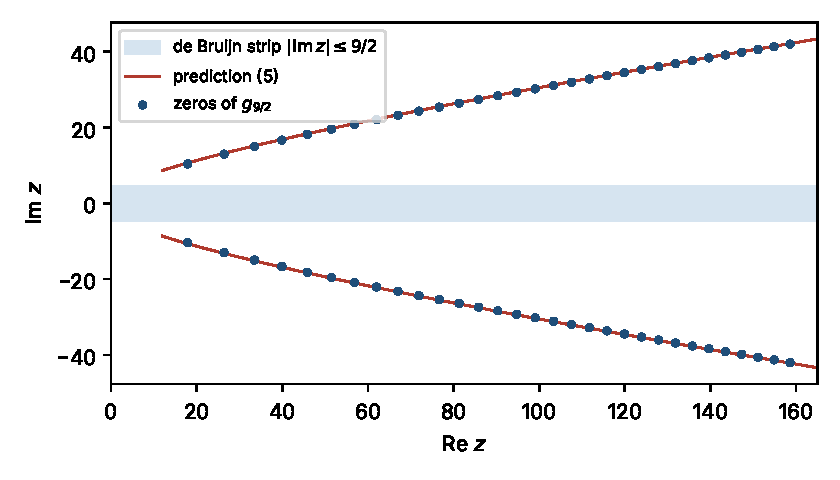
\includegraphics[width=\textwidth]{fig/mi_zeros.pdf}
\caption{The $31$ zeros of $g_{9/2}$ with real part below $160$ in the upper half plane of $z$ (circles), the escape law \eqref{mi:eq:escape} (curve), and the lines $|\im z|=\frac92$ bounding de Bruijn's strip $|\im w|\le\frac94$ in the scale $w=z/2$ of $g$ (dashed).}
\label{mi:fig:escape}
\end{figure}

For $b<2$ the root mean square de Bruijn radius of the P\'olya Gamma clock, $(\E\,4b^2\varpi)^{1/2}=b$, equals the strip width that de Bruijn's theorem needs for the shift identity. The strip nevertheless fails: below height $250$ the largest imaginary parts of zeros of $g_b$ are $0.367$, $1.258$, $2.153$ for $b=0.5$, $1$, $1.5$. Concentrating the clock does not help. Let $\varpi_h=\mathrm{PG}(h,0)/h$, so that $\E e^{-s\varpi_h}=\cosh(\sqrt{s/2h})^{-h}$ with mean $\frac14$; the corresponding weight at radius $b$ is $\sech(bu/\sqrt h)^h$, and $h\to\infty$ is the deterministic flow $\mathcal H_{-b^2/2}$. At radius $1$ the clocks $\mathrm{PG}(1)$, $\mathrm{PG}(4)$, $\mathrm{PG}(16)$ and the deterministic flow $\mathcal H_{-1/2}$ give $28$ nonreal pairs in $[0,250]\times[-3,3]$ for each (only $27$ of the pairs of $\mathrm{PG}(4)$ have imaginary part above $0.125$) and largest imaginary parts $1.258$, $1.331$, $1.322$, $1.325$. The obstruction is the backward direction of the flow, for which de Bruijn's radius has no counterpart.
